\documentclass[12pt]{article}
\usepackage{fullpage,enumitem,amsmath,amssymb,graphicx}
\usepackage{subcaption}
\usepackage{caption}
\usepackage{braket}
\usepackage{authblk}
\usepackage{tikz}
\usepackage{quantikz}
\usepackage{multicol}
\usepackage{float}
\renewcommand\Authfont{\bfseries}
\renewcommand\Affilfont{\small\ttfamily}

%\usepackage{indentfirst}
%\usepackage[hangul]{kotex}
\usepackage[
backend=biber,
style=numeric
]{biblatex}

\usepackage{hyperref} 
\hypersetup{
    colorlinks=true,
    linkcolor=blue,
    filecolor=magenta,      
    urlcolor=cyan,
}

\title{
    \textbf{QAMP 2025} \\        
    \vspace{0.5em}                            
    \small \textit{Enhancing Quantum Diffusion Models for Complex Image Generation}            
}



\addbibresource{bibliography.bib}

% author
\author[1]{Jeongbin Jo}
\author[2]{Santanam Wishal}
\author[3]{Shah Md Khalil Ullah}
\author[4]{Shan Kowalski}

% info.
\affil[1]{Department of Physics \\ Yonsei University \\ \textit{jeongbin033@yonsei.ac.kr}}
\affil[2]{Asia Cyber University \\ \textit{santawishal17@gmail.com}}
\affil[3]{Khulna University of Engineering and Technology \\ \textit{hamimkhandakar222@gmail.com}}
\affil[4]{Eleven Dimension LLC \\ \textit{shanjdk2012@gmail.com}}

%\newcommand{\pref}[1]{(\ref{#1})}
\begin{document}
\maketitle
\begin{abstract}
  In this study, we propose a Hybrid Quantum-Classical U-Net architecture designed for complex image generation.
  By integrating a classical encoder-decoder structure with a Quantum Bottleneck, 
  the model leverages the expressivity of quantum circuits while maintaining structural efficiency. 
  The architecture employs Skip Connections to preserve semantic information, which is critical for maintaining image sharpness.
\end{abstract}

\tableofcontents
\begin{center}

%\vspace{-0.3in}
%\begin{tabular}{rl}
%Collaborators: & 
%\end{tabular}
\end{center}



\noindent
\rule{\linewidth}{0.4pt}



%\begin{multicols}{2} % 2 block layout
  
\section{Intrduction}

Quantum Machine Learning (QML) is an emerging interdisciplinary research field that integrates principles of quantum computing with classical machine learning techniques to enhance data processing, pattern recognition, and optimization tasks. 
By exploiting quantum mechanical phenomena such as superposition, entanglement, and quantum interference, QML aims to provide computational advantages over classical learning algorithms, particularly for high-dimensional and complex datasets.

In classical machine learning, the performance of algorithms is often constrained by computational complexity and memory requirements as data size and model depth increase. 
Quantum computing, on the other hand, offers a fundamentally different computation paradigm, where information is represented using quantum bits (qubits) that can exist in multiple states simultaneously. 
This property allows quantum algorithms to explore large solution spaces more efficiently than their classical counterparts in certain scenarios.

One of the key motivations behind QML is the potential for speedup in tasks such as linear algebra operations, optimization, and sampling, which form the backbone of many machine learning models. 
Quantum-enhanced algorithms, including quantum support vector machines, variational quantum circuits, and quantum neural networks, have been proposed to accelerate learning processes and improve model expressiveness.

Despite its promising advantages, QML also faces several challenges. 
Current quantum hardware, commonly referred to as Noisy Intermediate-Scale Quantum (NISQ) devices, suffers from limited qubit counts, short coherence times, and gate errors. 
These hardware constraints restrict the depth and scalability of quantum models, often requiring hybrid quantum-classical approaches for practical implementations. 
Additionally, the theoretical quantum advantage of many QML algorithms remains an open research question, as classical algorithms continue to improve rapidly.

In summary, Quantum Machine Learning represents a promising yet evolving research direction. 
While it offers the potential for enhanced computational power and novel learning capabilities, significant challenges related to hardware limitations, noise, and algorithmic scalability must be addressed before widespread real-world adoption becomes feasible.


  \subsection{Quantum Convolutional Neural Network}



\section{Diffusion Model}
  \subsection{Classical Diffusion Model}
  Diffusion models are a class of generative models in machine learning inspired by non-equilibrium thermodynamics. The goal is to learn a diffusion process that destroys structure in data, and then learn a reverse process that restores structure to generate new data samples from noise.\cite{diffusion-model}

    \subsubsection{Forward Process: Diffusion Process}
    The forward process is defined by a Markov chain that gradually adds Gaussian noise to the data according to a variance schedule $\beta_1, \dots, \beta_T$.
    \begin{equation}
      q(x_t | x_{t-1}) = \mathcal{N}\left(x_t ; \sqrt{1-\beta_t}x_{t-1}, \beta_t \mathbf{I}\right)
    \end{equation}

    Using the notation $\alpha_t = 1 - \beta_t$ and $\bar{\alpha}_t = \prod_{s=1}^t \alpha_s$, we can sample $x_t$ at any arbitrary time step $t$ directly from $x_0$ in closed form:
    \begin{equation}
      q(x_t | x_0) = \mathcal{N}\left(x_t ; \sqrt{\bar{\alpha}_t}x_0, (1 - \bar{\alpha}_t)\mathbf{I}\right)
    \end{equation}
    This property allows for efficient training by eliminating the need to iterate through all previous timesteps.

    \subsubsection{Reverse Process: Generative Process}
    The generative process\cite{DBLP:journals/corr/abs-2006-11239} is defined as the reverse Markov chain. 
    Since the exact reverse posterior $q(x_{t-1}|x_t)$ is intractable, we approximate it using a neural network with parameters $\theta$:
    \begin{equation}
      p_\theta(x_{t-1} | x_t) = \mathcal{N}\left(x_{t-1} ; \mu_\theta(x_t, t), \Sigma_\theta(x_t, t) \right)
    \end{equation}
    Here, $\mu_\theta(x_t, t)$ is the predicted mean, and $\Sigma_\theta(x_t, t)$ is the covariance (often fixed to $\beta_t \mathbf{I}$ or learned).

    \subsubsection{Loss Function}
    Training is performed by optimizing the variational lower bound (VLB) on the negative log-likelihood.
    \begin{equation}
      \mathcal{L} = \mathbb{E} \left[ - \log p_\theta(\mathbf{x}_0) \right] \leq \mathbb{E}_q \left[ - \log \frac{p_\theta(\mathbf{x}_{0:T})}{q(\mathbf{x}_{1:T} | \mathbf{x}_0)} \right]
    \end{equation}

    This can be rewritten as a sum of KL divergence\cite{kl-divergence} terms:
    \begin{equation}
      \mathcal{L} = \mathbb{E}_q \left[ \underbrace{D_{KL}(q(\mathbf{x}_T|\mathbf{x}_0) || p(\mathbf{x}_T))}_{L_T} + \sum_{t>1} \underbrace{D_{KL}(q(\mathbf{x}_{t-1}|\mathbf{x}_t, \mathbf{x}_0) || p_\theta(\mathbf{x}_{t-1}|\mathbf{x}_t))}_{L_{t-1}} \underbrace{- \log p_\theta(\mathbf{x}_0|\mathbf{x}_1)}_{L_0} \right]
    \end{equation}

    In practice, Ho et al. found that a simplified objective function yields better sample quality. The objective is to predict the noise $\epsilon$ added to $x_0$:
    \begin{equation}
      \mathcal{L}_{\text{simple}}(\theta) = \mathbb{E}_{t, x_0, \epsilon} \left[ \| \epsilon - \epsilon_\theta(\sqrt{\bar{\alpha}_t}x_0 + \sqrt{1-\bar{\alpha}_t}\epsilon, t) \|^2 \right]
    \end{equation}
    where $\epsilon \sim \mathcal{N}(0, \mathbf{I})$ and $\epsilon_\theta$ is a function approximator (e.g., U-Net).

    \subsubsection{Continuous-Time Formulation: SDE}
    The discrete diffusion process can be generalized to continuous time using Stochastic Differential Equations (SDEs). 
    The forward process is described by the following It\^{o} SDE\cite{Ito-calculus}:
    \begin{equation}
      d\mathbf{x} = \mathbf{f}(\mathbf{x}, t)dt + g(t)d\mathbf{w}
    \end{equation}
    where $\mathbf{f}(\cdot, t)$ is the drift coefficient, $g(t)$ is the diffusion coefficient, and $\mathbf{w}$ is a standard Wiener process.

    Remarkably, the reverse process—generating data from noise—is also a diffusion process governed by the \textit{reverse-time SDE}\cite{ANDERSON1982313}:
    \begin{equation}
      d\mathbf{x} = \left[ \mathbf{f}(\mathbf{x}, t) - g(t)^2 \nabla_\mathbf{x} \log p_t(\mathbf{x}) \right] dt + g(t) d\bar{\mathbf{w}}
    \end{equation}
    Here, $dt$ represents a negative time step, and $\bar{\mathbf{w}}$ is the Brownian motion in reverse time. 
    The term $\nabla_\mathbf{x} \log p_t(\mathbf{x})$, known as the \textit{score function}, points towards high-density regions of the data.

    Therefore, the core task of the diffusion model is to learn a score-based model 
    $s_\theta(\mathbf{x}, t) \approx \nabla_\mathbf{x} \log p_t(\mathbf{x})$ using a neural network (or PQC in our case), 
    allowing us to numerically solve the reverse SDE to generate samples from noise.

  \subsection{Quantum Diffusion Model}
  While classical diffusion models operate on probability distributions over classical data, 
  Quantum Diffusion Models (QDMs) extend this concept to the Hilbert space of quantum states. 
  The goal is to generate quantum states (density matrices) from a maximally mixed state.

    \subsubsection{Forward Process: Depolarizing Channel}
    Instead of adding Gaussian noise, the forward process in QDM is typically modeled as a standard depolarizing channel acting on a density matrix $\rho$. 
    For a system of $n$ qubits with dimension $d=2^n$, the state at step $t$ is given by:

    \begin{equation}
      \rho_t = \mathcal{E}_t(\rho_{t-1}) = (1 - p_t)\rho_{t-1} + p_t \frac{I}{d}
    \end{equation}

    where $p_t \in [0, 1]$ is the depolarization probability (noise schedule). 
    Similar to the classical case, we can express $\rho_t$ directly from the initial state $\rho_0$. 
    Let $\alpha_t = \prod_{s=1}^t (1 - p_s)$, then:

    \begin{equation}
      \rho_t = \alpha_t \rho_0 + (1 - \alpha_t) \frac{I}{d}
    \end{equation}

    As $t \to T$, $\alpha_T \to 0$, and the state converges to the maximally mixed state $\rho_T \approx \frac{I}{d}$, 
    which contains no information about $\rho_0$.

    \subsubsection{Reverse Process: Quantum Denoising}
    The reverse process aims to restore the quantum state from the noise. 
    This is modeled by a parameterized quantum circuit (PQC), denoted as a unitary operator $U(\theta)$. 
    The discrete reverse step can be approximated as:

    \begin{equation}
      \rho_{t-1} \approx \mathcal{D}_\theta(\rho_t, t) = U(\theta_t) \rho_t U^\dagger(\theta_t)
    \end{equation}

    For more complex generative tasks, the reverse process may involve ancillary qubits and measurements to simulate non-unitary maps.

    \subsubsection{Loss Function: Fidelity or Trace Distance}
    Unlike the KL divergence used in classical models, 
    quantum models often use Fidelity or Hilbert-Schmidt distance to measure the closeness between the generated state and the target state. 
    A common objective is to maximize the overlap with the target pure state $\ket{\psi}$:

    \begin{equation}
      \mathcal{L}(\theta) = 1 - \mathbb{E} \left[ \bra{\psi} \rho_{\text{gen}}(\theta) \ket{\psi} \right]
    \end{equation}
    Alternatively, for density matrices, we minimize the trace distance or maximize the quantum fidelity $F(\rho, \sigma) = (\text{tr}\sqrt{\sqrt{\rho}\sigma\sqrt{\rho}})^2$.


\section{Quantum Data Encoding}
We referred to IBM Quantum Platform, especially Quantum Machine Learning.\cite{Data-encoding}
  \subsection{Basis Encoding}
  Basis encoding maps a classical $P$-bit string directly to a computational basis state of a $P$-qubit system. 
  For a single feature represented as binary bits $(b_1, b_2, \dots, b_P)$, the quantum state is:
  \begin{equation}
    \ket{x} = \ket{b_1, b_2, \dots, b_P}, \quad b_i \in \{0, 1\}
  \end{equation}

  \subsection{Amplitude Encoding}
  Amplitude encoding maps a normalized classical $N$-dimensional data vector $\vec{x}$ to the amplitudes of an $n$-qubit quantum state, 
  where $n = \lceil \log_2 N \rceil$.

  \begin{equation}
    \ket{\psi_x} = \frac{1}{\alpha}\sum_{i=1}^N x_i \ket{i}
  \end{equation}
  Here, $\ket{i}$ is the computational basis state and $\alpha$ is a normalization constant ensuring $\langle \psi_x | \psi_x \rangle = 1$. 
  And $\alpha$ is a normalization constant to be determined from the data being encoded. We use amplitude encoding in the quantum diffusion model.

  \begin{equation}
    \alpha = \sqrt{\sum_{i=1}^{N}|x_i|^2}
  \end{equation}

  \subsection{Angle Encoding}
  Angle encoding maps each feature $x_k$ to the rotation angle of a qubit using $R_Y$ gates. 
  For a data vector $\vec{x}$, the state is a product state:
  \begin{equation}
    \ket{\vec{x}} = \bigotimes_{k=1}^N R_Y(x_k)\ket{0} = 
    \bigotimes_{k=1}^N \left( \cos\left(\frac{x_k}{2}\right)\ket{0} + \sin\left(\frac{x_k}{2}\right)\ket{1} \right)
  \end{equation} 
  \subsection{Phase Encoding}
  Phase encoding maps data features to the phase of qubits using Phase gates $P(\phi)$, typically applied after Hadamard gates.
  \begin{equation}
    \ket{\vec{x}} = \bigotimes_{k=1}^N P(x_k)\ket{+} = 
    \frac{1}{\sqrt{2^N}} \bigotimes_{k=1}^N \left( \ket{0} + e^{i x_k}\ket{1} \right)  
  \end{equation} 

  \subsection{Dense Angle Encoding}
  Dense angle encoding encodes two features, $x_k$ and $x_l$, into a single qubit using both $Y$-axis and $Z$-axis rotations.
  \begin{equation}
    \ket{x_k, x_l} = R_Z(x_l) R_Y(x_k)\ket{0} = \cos\left(\frac{x_k}{2}\right)\ket{0} + e^{i x_l} \sin\left(\frac{x_k}{2}\right)\ket{1} 
  \end{equation}

  Extending this to more features, the data vector $\vec{x} = (x_1, ..., x_N)$ can be encoded as:
  \begin{equation}
    \ket{\vec{x}} = \bigotimes_{k=1}^{N/2}\left( \cos{x_{2k-1}}\ket{0} + e^{ix_{2k}}\sin{x_{2k-1}\ket{1}} \right)
  \end{equation}


\section{Quantum Circuit}
The choice of quantum circuit ansatz is critical in designing Quantum Machine Learning (QML) models, 
as it determines the expressivity and trainability of the network within the constraints of Noisy Intermediate-Scale Quantum (NISQ) devices. 
Based on recent surveys and specific applications in diffusion models, we categorize relevant ansatzes into general-purpose architectures and task-specific designs for image processing.

\subsection{General Variational Ansatzes}
\begin{itemize}
    \item \textbf{Hardware-Efficient Ansatz (HEA):} 
    Designed to minimize circuit depth and gate count on NISQ devices, HEA utilizes a layered structure of parameterized single-qubit rotations followed by entangling gates (e.g., CNOTs) tailored to the specific connectivity of the quantum hardware \cite{guo2024patterns}. While it offers high implementability, it is known to suffer from barren plateaus if not carefully initialized.
    
    \item \textbf{Hamiltonian Variational Ansatz (HVA):} 
    Inspired by the Quantum Approximate Optimization Algorithm (QAOA) and adiabatic quantum computation, HVA constructs the ansatz based on the problem Hamiltonian. It is particularly effective for physics-inspired problems but introduces a hierarchical structure to manage complexity \cite{guo2024patterns}.
\end{itemize}

\subsection{Ansatzes for Quantum Machine Learning and Vision}
For high-dimensional data such as images, specialized ansatzes inspired by tensor networks and convolutional neural networks are preferred.

\begin{itemize}
    \item \textbf{Quantum Convolutional Neural Network (QCNN):} 
    QCNN adapts the structure of classical CNNs to the quantum domain. It consists of alternating convolutional layers (quasilocal unitary evolutions) and pooling layers (measurements or partial traces) to hierarchically reduce dimensionality while extracting features \cite{guo2024patterns}. This structure effectively captures spatial correlations, making it suitable for image generation tasks.
    
    \item \textbf{Multiscale Entanglement Renormalization Ansatz (MERA):} 
    Originally designed for simulating quantum many-body systems, MERA represents quantum states using a hierarchical tensor network. It efficiently captures correlations at different length scales, which is analogous to the feature extraction process in deep learning \cite{guo2024patterns}.
\end{itemize}

\subsection{Optimal General Two-Qubit Ansatz (Vatan-Williams Decomposition)}


We adopt the optimal quantum circuit decomposition for general two-qubit interactions as proposed by Vatan and Williams \cite{Vatan_2004}. Specifically, we utilize the explicit circuit construction for the non-local interaction block $N(\alpha, \beta, \gamma)$, which is the core component of the ansatz.

The circuit structure, depicted in Fig.~\ref{fig:interaction_block}, consists of three CNOT gates interleaved with parameterized single-qubit rotations. This configuration is capable of simulating the unitary operator $U = \exp(-i(\alpha \sigma_x \otimes \sigma_x + \beta \sigma_y \otimes \sigma_y + \gamma \sigma_z \otimes \sigma_z))$ up to local basis transformations.

\begin{figure}[h]
    \centering
    \begin{quantikz}
        \lstick{$q_0$} & \qw & \targ{} & \gate{R_z(\frac{\pi}{2}-2\gamma)} & \ctrl{1} & \qw & \targ{} & \gate{R_z(\frac{\pi}{2})} & \qw \\
        \lstick{$q_1$} & \gate{R_z(-\frac{\pi}{2})} & \ctrl{-1} & \gate{R_y(2\alpha-\frac{\pi}{2})} & \targ{} & \gate{R_y(\frac{\pi}{2}-2\beta)} & \ctrl{-1} & \qw & \qw
    \end{quantikz}
    \caption{The parameterized quantum circuit used in our Quantum Bottleneck. This structure implements the optimal decomposition for arbitrary two-qubit entangling gates, characterized by the parameters $\alpha, \beta, \gamma$. Note the alternating CNOT direction and the specific rotation angles derived from the canonical decomposition.}
    \label{fig:interaction_block}
\end{figure}

The parameters $\alpha, \beta, \gamma$ serve as the learnable weights of the quantum diffusion model, allowing the network to capture complex correlations between features represented by qubits $q_0$ and $q_1$.

\subsection{Global Correlation and Phase Mixing}

While the convolutional layers capture local spatial dependencies, generating high-fidelity images requires the model to understand global structures and high-frequency details. To address this, we introduce a \textit{Phase Mixing} block designed to enhance the expressivity of the ansatz in the frequency domain \cite{schuld2021effect}.

The Phase Mixing block consists of two stages:
\begin{enumerate}
    \item \textbf{Star-Topology Entanglement:} We apply a series of Controlled-Rotation $Z$ ($CRZ$) gates. As shown in the code implementation, the first qubit ($q_0$) acts as a central node (control), interacting with all other qubits ($q_i$) via parameterized rotations. This creates a "star" connectivity graph, efficiently distributing information from the central feature to the entire register.
    \item \textbf{Quantum Fourier Transform (QFT):} Following the entanglement, a QFT operation is applied to the register. This transforms the encoded information from the computational basis to the Fourier basis, effectively mixing the local correlations into global phase information \cite{nielsen2010quantum}.
\end{enumerate}

The circuit diagram for this block is illustrated in Fig.~\ref{fig:phase_mixing}.

\begin{figure}[h]
    \centering
    \begin{quantikz}
        \lstick{$q_0$} & \ctrl{1} & \ctrl{2} & \qw & \dots & \ctrl{3} & \gate[4, disable auto height]{QFT} & \qw \\
        \lstick{$q_1$} & \gate{R_z(\phi_1)} & \qw & \qw & \dots & \qw & \qw & \qw \\
        \lstick{$q_2$} & \qw & \gate{R_z(\phi_2)} & \qw & \dots & \qw & \qw & \qw \\
        \vdots & & & & \ddots & & & \\
        \lstick{$q_{n-1}$} & \qw & \qw & \qw & \dots & \gate{R_z(\phi_{n-1})} & \qw & \qw
    \end{quantikz}
    \caption{The \textit{Phase Mixing} architecture. It employs a star-topology interaction where the first qubit controls parameterized $R_z$ rotations on all other qubits, followed by a Quantum Fourier Transform (QFT) to enforce global mixing. This structure allows the model to learn complex frequency-domain features essential for image sharpness.}
    \label{fig:phase_mixing}
\end{figure}

Mathematically, this operation can be expressed as:
\begin{equation}
    U_{\text{mix}}(\vec{\phi}) = \text{QFT} \cdot \prod_{i=1}^{n-1} CRZ_{0 \to i}(\phi_i)
\end{equation}
where $CRZ_{c \to t}(\phi) = |0\rangle\langle 0|_c \otimes I_t + |1\rangle\langle 1|_c \otimes R_z(\phi)_t$.



\section{Adaptive Non-Local Measurement}

In conventional Variational Quantum Circuits (VQCs), information extraction is typically limited to fixed local measurements, such as the expectation values of Pauli-$Z$ operators ($\langle \sigma_z^{(i)} \rangle$). 
This approach restricts the accessible information to local properties of individual qubits, failing to capture the rich correlations encoded in the entangled quantum state.

To fully leverage the high-dimensional Hilbert space of our quantum bottleneck, we implement the \textit{Adaptive Non-Local Observable (ANO)} framework \cite{lin2026quantumsuperresolutionadaptivenonlocal}. 
Instead of fixed operators, we employ a set of trainable Hermitian observables $\{H_k\}_{k=1}^{K}$ that act on the entire qubit register.

\subsection{Trainable Hermitian Construction}
For an $n$-qubit system with dimension $D=2^n$, a general observable is represented by a $D \times D$ Hermitian matrix. We parameterize the $k$-th observable $H_k(\phi_k)$ using a complex matrix $M_k(\phi_k) \in \mathbb{C}^{D \times D}$ with learnable weights $\phi_k$:
\begin{equation}
    H_k(\phi_k) = \frac{1}{2} \left( M_k(\phi_k) + M_k(\phi_k)^\dagger \right)
\end{equation}
This construction guarantees the Hermiticity ($H = H^\dagger$) required for valid quantum measurements while allowing the optimization process to explore the full manifold of observable operators.

\subsection{High-Dimensional Feature Extraction}
A key advantage of our approach is the ability to decouple the output feature dimension $K$ from the number of physical qubits $n$. By configuring $K \ge n$, we can extract an over-complete set of features from the latent quantum state $\rho = |\psi(\theta)\rangle\langle\psi(\theta)|$. 
The output vector $\mathbf{y} \in \mathbb{R}^K$ fed into the classical decoder is given by:
\begin{equation}
    y_k = \langle \psi(\theta) | H_k(\phi_k) | \psi(\theta) \rangle = \text{Tr}(\rho H_k(\phi_k)), \quad k=1, \dots, K
\end{equation}
By jointly training the circuit parameters $\theta$ and the measurement parameters $\phi$, the model learns to construct "quantum lenses" that focus on the specific sub-spaces containing the most relevant features for image reconstruction, such as high-frequency edge details.


\begin{figure}[t]
    \centering
    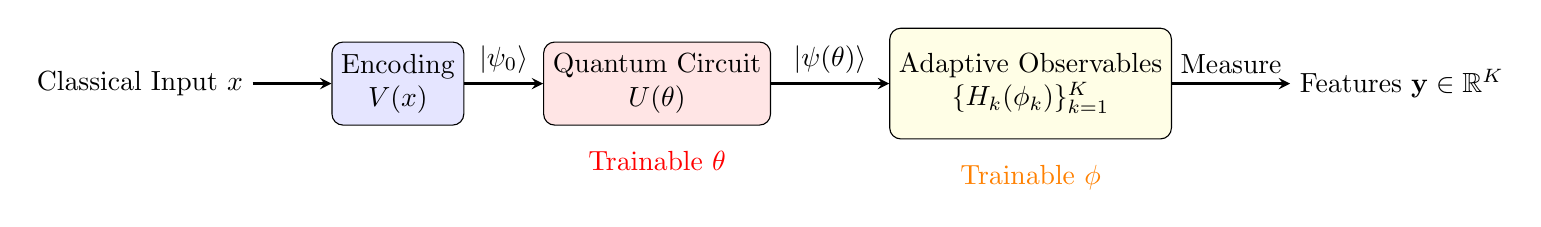
\begin{tikzpicture}
        % Define styles
        \tikzstyle{block} = [draw, rectangle, minimum height=3em, minimum width=3em, align=center, rounded corners]
        \tikzstyle{arrow} = [thick,->,>=stealth]
        
        % Nodes
        \node (input) {Classical Input $x$};
        \node[block, fill=blue!10, right=1cm of input] (encoder) {Encoding \\ $V(x)$};
        \node[block, fill=red!10, right=1cm of encoder] (ansatz) {Quantum Circuit \\ $U(\theta)$};
        
        % ANO Part
        \node[block, fill=yellow!10, right=1.5cm of ansatz, minimum height=4em] (ano) {Adaptive Observables \\ $\{H_k(\phi_k)\}_{k=1}^K$};
        
        \node[right=1.5cm of ano] (output) {Features $\mathbf{y} \in \mathbb{R}^K$};
        
        % Arrows
        \draw[arrow] (input) -- (encoder);
        \draw[arrow] (encoder) -- node[above] {$|\psi_0\rangle$} (ansatz);
        \draw[arrow] (ansatz) -- node[above] {$|\psi(\theta)\rangle$} (ano);
        \draw[arrow] (ano) -- node[above] {Measure} (output);
        
        % Annotations for Learnable Params
        \node[below=0.2cm of ansatz, text=red] {Trainable $\theta$};
        \node[below=0.2cm of ano, text=orange] {Trainable $\phi$};
        
    \end{tikzpicture}
    
    \caption{Schematic of the Quantum Bottleneck with Adaptive Non-Local Observables (ANO). 
    Unlike standard VQCs that output $N$ local measurements, our ANO framework employs a set of $K$ trainable Hermitian operators $\{H_k(\phi_k)\}$. 
    This allows the extraction of high-dimensional feature vectors ($K \ge N$) from the entangled quantum state $|\psi(\theta)\rangle$, effectively acting as a learnable quantum lens for super-resolution tasks.}
    \label{fig:ano_architecture}
\end{figure}
% \subsection{Architectures for Diffusion and Super-Resolution}
% Recent studies on quantum generative models have introduced specialized architectures to enhance training stability and resolution.

% \begin{itemize}
%     \item \textbf{Reverse-Bottleneck PQC:} 
%     In the context of Quantum Diffusion Models, Cacioppo et al. proposed the \textit{Reverse-Bottleneck} architecture. Unlike standard bottleneck designs, this approach introduces ancillary qubits and performs measurements in a specific order (reversing the ancilla introduction) to maintain the flow of information during the denoising steps \cite{cacioppo2023diffusion}. This structure has shown superior performance in generating coherent samples compared to standard designs.
    
%     \item \textbf{Adaptive Non-Local Observables (ANO):} 
%     To overcome the resolution limits of fixed Pauli measurements, Lin et al. proposed the ANO framework. Instead of fixed observables, ANO employs trainable multi-qubit Hermitian operators. This allows the measurement process itself to adapt during training, effectively acting as a high-resolution lens that extracts fine-grained information from the entangled quantum state \cite{lin2026sr}.
% \end{itemize}

\section{Circuit Benchmarking and Evaluation}

Before integrating the Quantum Bottleneck into the full U-Net architecture, we quantitatively evaluated the intrinsic properties of our proposed ansatz. 
Following the framework established by Sim et al. \cite{Sim_2019}, we utilize two key descriptors: \textit{Expressibility} and \textit{Entangling Capability}. 
These metrics ensure that our circuit is sufficiently expressive to model complex latent distributions while effectively capturing non-local correlations required for the diffusion process.

\subsection{Expressibility via KL Divergence}

Expressibility measures the ability of a parameterized quantum circuit (PQC) to explore the Hilbert space. We quantify this by comparing the distribution of state fidelities generated by our ansatz against the distribution expected from an ensemble of Haar-random states (which represents the maximally expressive uniform distribution).

Let $F = |\langle \psi_{\theta} | \psi_{\phi} \rangle|^2$ be the fidelity between two states sampled from the PQC with random parameters $\theta, \phi$. The probability density function (PDF) of fidelities for Haar-random states in an $N$-dimensional Hilbert space ($N=2^n$) is given by $P_{\text{Haar}}(F) = (N-1)(1-F)^{N-2}$.

The expressibility $E$ is defined as the Kullback-Leibler (KL) divergence between the PQC's fidelity distribution $P_{\text{PQC}}(F)$ and the analytical Haar distribution $P_{\text{Haar}}(F)$:
\begin{equation}
    E = D_{KL}(P_{\text{PQC}} || P_{\text{Haar}}) = \int_0^1 P_{\text{PQC}}(F) \ln \left( \frac{P_{\text{PQC}}(F)}{P_{\text{Haar}}(F)} \right) dF
\end{equation}
A lower value of $E$ indicates that the ansatz can uniformly explore the Hilbert space, approaching the statistical properties of random states. In our experiments, we approximate this integral using a discretized histogram of sampled fidelities.

\subsection{Entangling Capability via Meyer-Wallach Measure}

To verify the circuit's ability to generate multi-partite entanglement—a crucial feature for capturing global dependencies in image data—we employ the Meyer-Wallach (MW) measure $Q$. For a given state $|\psi\rangle$, the MW measure is defined as the average purity of the single-qubit reduced density matrices:
\begin{equation}
    Q(|\psi\rangle) = \frac{4}{n} \sum_{k=1}^{n} D(\iota_k(|\psi\rangle)) = \frac{4}{n} \sum_{k=1}^{n} \frac{1}{2} \left( 1 - \text{Tr}(\rho_k^2) \right)
\end{equation}
where $\rho_k = \text{Tr}_{\neg k}(|\psi\rangle\langle\psi|)$ is the reduced density matrix of the $k$-th qubit. The value $Q$ ranges from 0 (product states, unentangled) to 1 (maximally entangled, e.g., GHZ states).

We estimate the \textit{Entangling Capability} of our ansatz by averaging $Q$ over an ensemble of states sampled with uniformly random parameters:
\begin{equation}
    \bar{Q} = \frac{1}{S} \sum_{i=1}^{S} Q(|\psi(\theta_i)\rangle)
\end{equation}
A high $\bar{Q}$ value confirms that our \textit{ConvUnit} and \textit{PhaseMixing} layers successfully distribute information across the qubit register, facilitating the "global mixing" required for high-resolution image synthesis.

\subsection{Visualizing the State Space}
In addition to quantitative metrics, we visualize the distribution of single-qubit reduced states on the Bloch sphere. 
As shown in Fig.~\ref{fig:bloch_dist}, the concentration of states within the interior of the Bloch sphere (as opposed to the surface) serves as visual evidence of entanglement, consistent with high Meyer-Wallach values.

\begin{figure}[H]
    \centering
    \includegraphics[width=0.85\linewidth]{figure/bloch_sphere_dist.png}
    \caption{Visualization of the single-qubit reduced state distribution on the Bloch sphere generated by our ANO-based ansatz. 
    Each red point represents the state of the first qubit traced out from the multi-qubit system, sampled over random circuit parameters. 
    (Left) Points distributed strictly on the surface indicate product states with no entanglement. 
    (Right) Points filling the interior volume demonstrate the generation of strong multi-partite entanglement, as the reduced state becomes mixed due to correlations with other qubits. 
    This volumetric coverage visually corroborates the high Meyer-Wallach measure and Expressibility scores.}
    \label{fig:bloch_dist}
\end{figure}


\subsection{Architecture}
The proposed model, illustrated in Figure \ref{fig:architecture}, 
adopts a hybrid quantum-classical U-Net architecture inspired by recent advances in quantum generative diffusion models\cite{cacioppo2023quantumdiffusionmodels, qdm}. 
The architecture is designed to leverage the expressivity of quantum circuits while maintaining the reconstruction capability of classical networks. 
It consists of three distinct modules: a classical encoder, a quantum bottleneck (core), and a classical decoder.

\begin{figure}[htbp]
  \centering
  \includegraphics[width=\linewidth]{figure/QuantumUNet_Final_LR.png}
  \caption{Schematic of the Hybrid Quantum-Classical U-Net Architecture. The model integrates a quantum bottleneck for feature extraction and employs a skip connection to preserve original semantic information during the reverse diffusion process.}
  \label{fig:architecture}
\end{figure}

First, the \textbf{Classical Encoder} transforms the input data (flattened vector) into a lower-dimensional latent representation. 
To seamlessly interface with the quantum layer, we utilize complex-valued linear layers (\texttt{ComplexLinear}) that preserve phase information necessary for quantum state preparation.

Second, the \textbf{Quantum Bottleneck} acts as the core generative component. 
We employ \textit{amplitude encoding} to efficiently map the classical latent vector $\mathbf{z}$ onto an $n$-qubit quantum state $|\psi\rangle$ by normalizing the complex vector. 
This state is evolved by a Parameterized Quantum Circuit (PQC), $U(\theta)$, which learns the reverse diffusion dynamics. 
The resulting quantum state is then measured to extract quantum features (Q-Feats).

Finally, the \textbf{Classical Decoder} reconstructs the denoised sample from the quantum features. 
A crucial design element is the inclusion of a \textbf{Skip Connection} (red path in Figure \ref{fig:architecture}). 
This connection concatenates the original flattened input vector directly with the quantum features in the decoder. 
This mechanism is essential for mitigating the "bottleneck" problem inherent in low-qubit quantum circuits and preventing the model from converging to trivial identity mappings by preserving the original signal structure.

\section{Experimental Results}

We evaluated the proposed Hybrid Quantum U-Net using the MNIST dataset. 
The training was conducted for 100 epochs, and the model demonstrated stable convergence behavior. 
As shown in Figure \ref{fig:loss}, the final infidelity loss reached approximately 0.25. 
Remarkably, the total execution time was only about 3 minutes, highlighting the computational efficiency of our hybrid architecture compared to fully classical counterparts or more complex quantum simulations.

\begin{figure}[htbp]
  \centering
  \includegraphics[width=0.6\linewidth]{figure/loss.png}
  \caption{Training Loss Convergence. The model achieves a stable loss of $\approx 0.25$ within 100 epochs, demonstrating rapid convergence.}
  \label{fig:loss}
\end{figure}

Figure \ref{fig:forward} visualizes the forward diffusion process used in our experiment. 
The input data is gradually corrupted by adding Gaussian noise over discrete time steps $t$, eventually converging to an isotropic Gaussian distribution.

\begin{figure}[htbp]
  \centering
  \includegraphics[width=\linewidth]{figure/forward.png}
  \caption{Visualization of the Forward Diffusion Process. The original digits (left) are progressively transformed into random noise (right).}
  \label{fig:forward}
\end{figure}

To analyze the generative capability and scalability of the model, 
we compared two scenarios: a low-complexity subset (digits 0 and 1) and the full dataset (digits 0 through 9). 
The generation results are presented in Figure \ref{fig:gen}.

\begin{figure}[htbp]
  \centering
  \begin{subfigure}[b]{0.48\textwidth}
    \centering
    \includegraphics[width=\linewidth]{figure/trial1.png}
    \caption{Binary Class (Digits 0, 1)} 
    \label{fig:trial1}
  \end{subfigure}
  \hfill
  \begin{subfigure}[b]{0.48\textwidth}
    \centering
    \includegraphics[width=\linewidth]{figure/trial2.png}
    \caption{Multi-Class (Digits 0-9)} 
    \label{fig:trial2}
  \end{subfigure}
  \caption{Comparison of Generated Samples. (a) shows sharp features for the binary case, while (b) exhibits increased ambiguity and blurring due to higher data complexity.}
  \label{fig:gen}
\end{figure}

As observed in Figure \ref{fig:trial1}, the model successfully generates distinct and sharp images when trained on binary classes. 
However, as the complexity increases to include all ten digits (Figure \ref{fig:trial2}), the generated samples exhibit ambiguous shapes and blurring. 
This suggests that while the current quantum bottleneck is efficient, its limited Hilbert space (number of qubits) constrains the expressibility required to fully capture the complex multimodal distribution of the entire dataset.


\section{Conclusion}
In this study, we proposed a \textbf{Hybrid Quantum-Classical U-Net} architecture 
for complex image generation and validated its effectiveness using the MNIST dataset. 
The experimental results demonstrated that the proposed model exhibits significant generative capabilities with a reduced number of parameters, confirming the potential of hybrid structures in the NISQ era. 
The key insights gained, technical challenges faced, and our current research direction are summarized below.

\subsection*{Key Insights and Learnings}
\begin{itemize}
    \item \textbf{Structural Efficiency:} 
    Through code implementation (\texttt{QuantumUNet}), we verified that the `Quantum Bottleneck' architecture—which compresses features via a classical encoder before mapping them to a quantum state is significantly more efficient than encoding the entire high-dimensional image directly into qubits.
    \item \textbf{Importance of Skip Connections:} 
    We discovered that \textbf{Skip Connections}, which combine original classical features with quantum features in the decoder stage, are critical. Without them, the information loss inherent in the quantum circuit significantly degrades image sharpness. 
    This highlights that preserving the \textbf{Classical Path} is essential for maintaining reconstruction quality in hybrid models.
\end{itemize}

\subsection*{Technical Challenges}
\begin{itemize}
    \item \textbf{Simulation Overhead (Running Speed):} 
    A major practical barrier was the \textbf{ML running speed}. Simulating quantum circuits (especially tensor product operations for entanglement) on classical hardware incurs massive computational costs. 
    This overhead severely constrained our ability to scale up the number of qubits and circuit depth within a reasonable training time.
    \item \textbf{Barren Plateaus \& Optimization Landscape:} 
    Beyond computational speed, we faced the fundamental challenge of \textbf{Barren Plateaus}. 
    The standard Adam optimizer struggled to navigate the flat loss landscapes typical of parameterized quantum circuits (PQCs). 
    This often led to stagnation or convergence to local minima, particularly when attempting to learn the complex multi-modal distributions of the multi-class MNIST dataset.
\end{itemize}

\subsection*{Current Status: Enhancing Optimization with QNGD}
To address these optimization challenges and ensure convergence stability, we are currently implementing \textbf{Quantum Natural Gradient Descent (QNGD)}.

\begin{itemize}
    \item \textbf{Addressing the Optimization Geometry:} 
    Standard optimizers like Adam assume a Euclidean parameter space, which is ill-suited for the quantum state space that follows Riemannian geometry. 
    We are adopting QNGD to adjust the gradient direction by incorporating the \textbf{Fubini-Study Metric Tensor} ($g_{ij}$), which represents the curvature of the quantum information geometry. 
    The update rule is defined as:
    \begin{equation}
        \theta_{t+1} = \theta_t - \eta g^{-1}(\theta_t) \nabla \mathcal{L}(\theta_t)
    \end{equation}
    where $\eta$ is the learning rate and $g^{-1}(\theta_t)$ corrects the gradient based on the local curvature.
    
    \item \textbf{Quality over Speed (Trade-off):} We acknowledge that calculating the metric tensor increases the computational cost per step, potentially lengthening the wall-clock training time. 
    However, we accept this trade-off to \textbf{mitigate Barren Plateaus} and achieve higher \textbf{Fidelity} with fewer training epochs. 
    Our focus has shifted from raw simulation speed to \textbf{`Optimization Efficiency'}, aiming to overcome the expressivity and convergence limitations of the current model.
\end{itemize}


\printbibliography
% \end{multicols} % 2 block layout

\end{document}
